\documentclass{article}
\usepackage{tikz}
\usetikzlibrary{arrows.meta,positioning,calc,shapes.geometric}
\pagestyle{empty}
\begin{document}
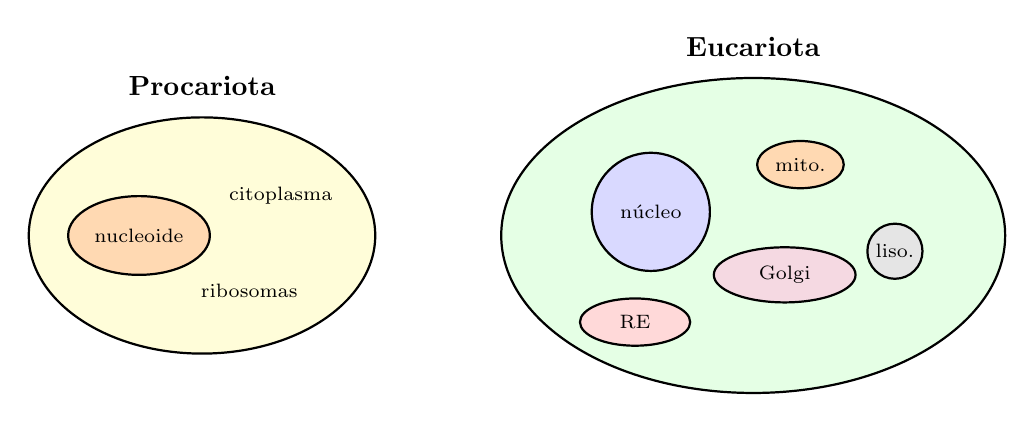
\begin{tikzpicture}

\draw[thick, fill=yellow!15] (0,0) ellipse (2.2 and 1.5);
\node[font=\bfseries] at (0,1.9) {Procariota};
\draw[thick, fill=orange!30] (-0.8,0) ellipse (0.9 and 0.5); \node[font=\scriptsize] at (-0.8,0) {nucleoide};
\node[font=\scriptsize, align=center] at (0.6,-0.7) {ribosomas};
\node[font=\scriptsize] at (1.0,0.5) {citoplasma};
\draw[thick, fill=green!10] (7,0) ellipse (3.2 and 2.0);
\node[font=\bfseries] at (7,2.4) {Eucariota};
\draw[thick, fill=blue!15] (5.7,0.3) circle (0.75); \node[font=\scriptsize] at (5.7,0.3) {núcleo};
\draw[thick, fill=orange!30] (7.6,0.9) ellipse (0.55 and 0.3); \node[font=\scriptsize] at (7.6,0.9) {mito.};
\draw[thick, fill=purple!15] (7.4,-0.5) ellipse (0.9 and 0.35); \node[font=\scriptsize] at (7.4,-0.5) {Golgi};
\draw[thick, fill=red!15] (5.5,-1.1) ellipse (0.7 and 0.3); \node[font=\scriptsize] at (5.5,-1.1) {RE};
\draw[thick, fill=gray!20] (8.8,-0.2) circle (0.35); \node[font=\scriptsize] at (8.8,-0.2) {liso.};

\end{tikzpicture}
\end{document}
